\documentclass[10pt,a4paper]{article}
\usepackage[utf8]{inputenc}
\usepackage[francais]{babel}
\usepackage[T1]{fontenc}
\usepackage{amsmath}
\usepackage{amsfonts}
\usepackage{amssymb}
\usepackage{makeidx}
\usepackage{graphicx}
\usepackage{float} %pour que l'option "H" fonctionne dans figure.
\usepackage[left=2cm,right=2cm,top=2cm,bottom=2cm]{geometry}
\usepackage{hyperref} % lien hypertext
%\hypersetup{pdfborder={0 0 0}}

\begin{document}
%\setcounter{page}{1} % enlever numero de page


\begin{minipage}{0.5\linewidth} % permet de faire les deux colonnes pour mettre l'image à  droite du texte
Colpier Clément\\
Fornara Thibault\\
Pellegrino Guillaume\\
Renard Charles\\



26/01/13
\end{minipage}
\begin{minipage}{0.5\linewidth}
\begin{flushright}

\includegraphics[scale=0.2]{logo-esiee.jpg}

\end{flushright}
\end{minipage}


\vspace{8cm}

\begin{center}
\LARGE Projet de Mathématiques appliquées \\
\-
\LARGE PR3003
\\

\end{center}




\newpage
-
\newpage
\tableofcontents              % Table des matieres
\clearpage


\section{Déterminer l'équation différentielle vérifiée par M(t)=(x(t),y(t)).}
\begin{figure}[H]
	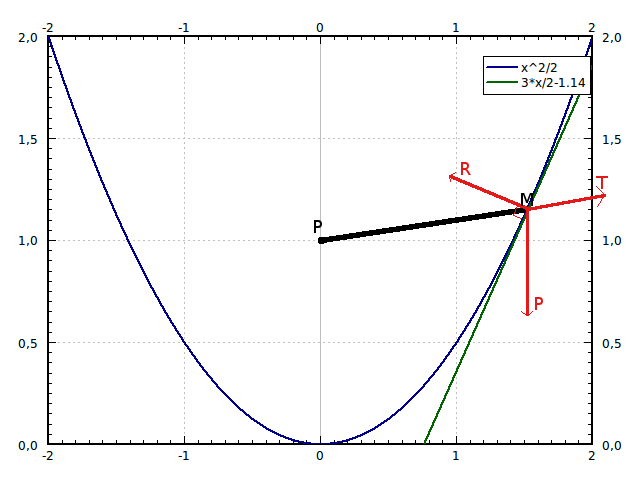
\includegraphics[scale=0.7]{GraphMath2.png}
	%\caption{Histoire de Sanofi}
\end{figure}
La masselotte M se déplace uniquement selon la composante tangentielle. Pour déterminer l'équation différentielle on va donc particulièrement s'intéresser à l'équation sur la composante tangentielle.\\
Pour cela, on commence à faire la somme des forces s'exerçant sur la composante tangentielle $\vec{u_t}$ et normale $\vec{u_n}$ selon la seconde loi de Newton (PFD) :
\[
   \left \{
   \begin{array}{r c l}
      P_t+T_t=ma_t  \\
      P_n+R_n+T_n=0 
   \end{array}
   \right .
\]
On s'intéresse à l'équation: \[\fbox{$P_t+T_t=ma_t$}\] \\ 
Pour déterminer l'équation différentielle, on doit alors projeter $\vec{T}$ et  $\vec{mg}$ sur $\vec{u_t}$. \\
On projette $\vec{mg}=-mg.\vec{u_y}$ sur $\vec{u_t}$\\

\subsection{Projection du Poids sur la composante tangentielle}
\begin{figure}[H]
	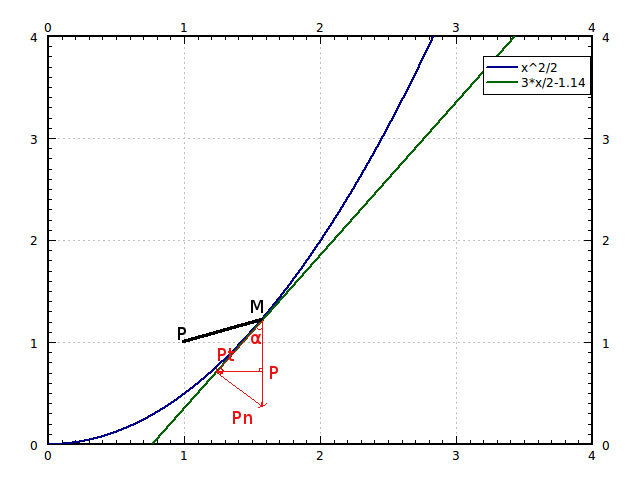
\includegraphics[scale=0.7]{GraphMathZoomProjectionPoids.png}
	%\caption{Histoire de Sanofi}
\end{figure}

On remarque sur le graphique que $P_t=P.\cos(\alpha)$\\
On cherche à déterminer $\alpha$.
On calcule la pente a de la tige parabolique. $a=\frac{\partial y}{\partial x}=\frac{\partial x^2/2}{\partial x}=x$ \\
En $M(x_0,y_0)$ la pente a de la tige parabolique vaut donc $x_0$.
Cette pente a nous permet de calculer l'angle $\alpha$. En effet, on remarque graphiquement que $\tan(\alpha)=\frac{1}{a}$. On en déduit: $\alpha=\tan^{-1}(\frac{1}{x_0})$\\
Au final on trouve donc: $P_t=P.\cos(\tan^{-1}(\frac{1}{x_0})) $\\
Or $\cos(\tan^{-1}(x))=\frac{1}{\sqrt{1+x^2}}$  On en déduit donc: $P_t=P.\frac{1}{\sqrt{1+1/x^2_0}}$ D'où: 
\[\fbox{$P_t=P.\frac{x_0}{\sqrt{1+x^2_0}}$}\]

\subsection{Projection de la tension du ressort su la composante tangentielle}
On projette désormais $\vec{T}$ sur $\vec{u_t}$.\\
\subsubsection{Methode de Guillaume, diff d'angle}
\begin{figure}[H]
	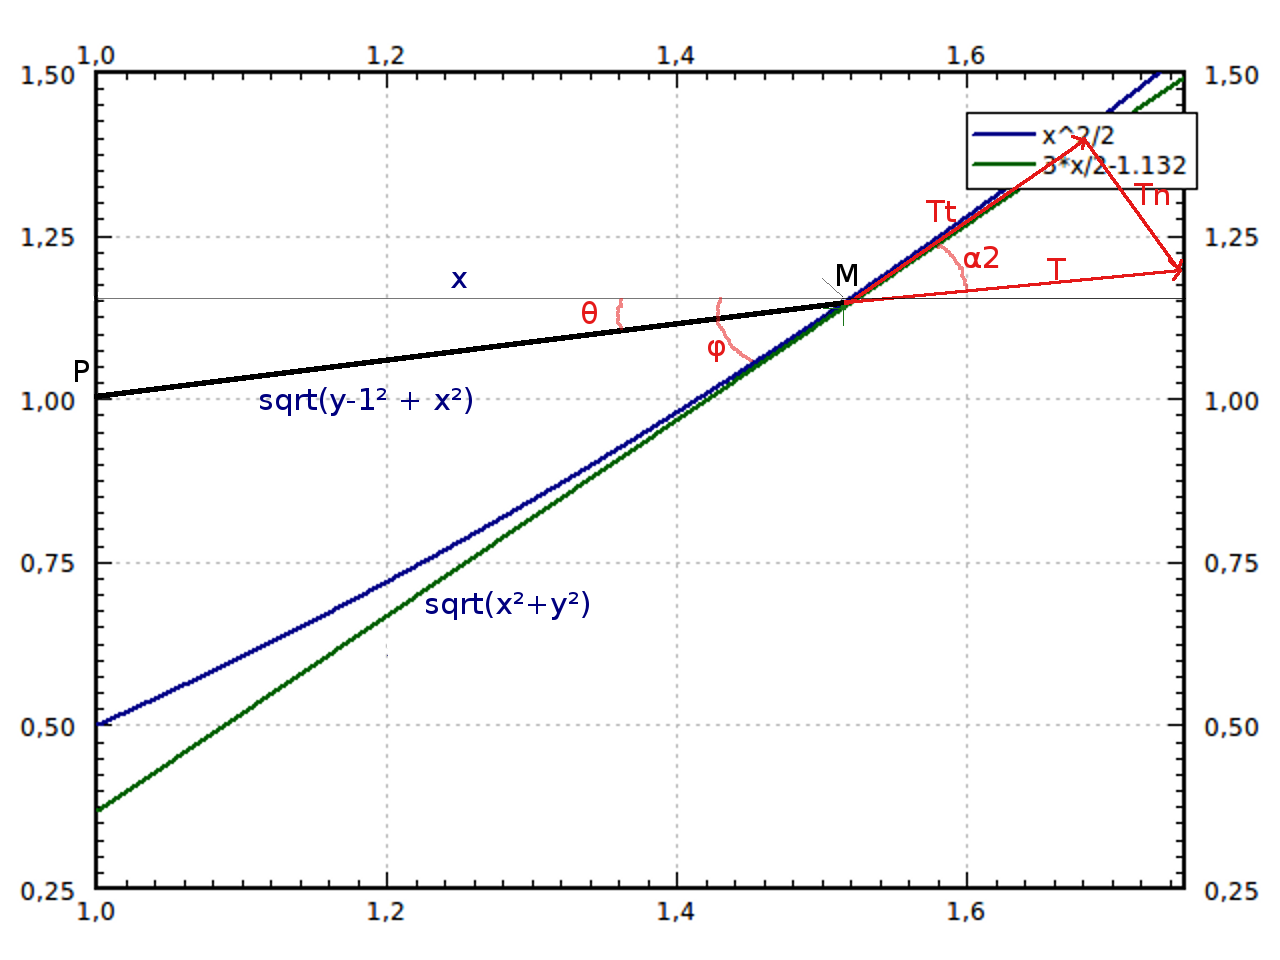
\includegraphics[scale=0.35]{GraphMathZoomProjectionT2.png}
	%\caption{Histoire de Sanofi}
\end{figure} 
$\cos(\phi)=\frac{x}{\sqrt{x^2+y^2}}=\frac{1}{\sqrt{1+x^2}}$ \\

$\cos(\theta)=\frac{x}{\sqrt{(1-y)^2+x^2}}=\frac{x}{\sqrt{1+x^4/4}}$ \\
Et: 
$T_t=T.\cos(\alpha 2)=T.\cos(\phi - \theta)=T[\cos(\phi).\cos(\theta)+\sin(\phi).\sin(\theta)]$\\
On en déduit:\\
$T_t=T[\frac{1}{\sqrt{1+x^2}}.\frac{x}{\sqrt{1+x^4/4}} + \sin(\cos^{-1}(\frac{1}{\sqrt{1+x^2}})).\sin(\cos^{-1}(\frac{x}{\sqrt{1+x^4/4}}))]$\\
Or: $\sin(\cos^{-1}(u))=\sqrt{1-u^2}$\\
On trouve donc:\[\fbox{$T_t=T.[\frac{1}{\sqrt{1+x^2}}.\frac{x}{\sqrt{1+x^4/4}} + \sqrt{1-\frac{1}{1+x^2}}.\sqrt{1-\frac{x^2}{1+x^4/4}}]$}\]\\

%La pente de la tangente vaut $x_0$. Celle de $\vec{PM}$ vaut $\frac{y_0-1}{x_0}$.\\
%On en déduit ainsi: $\tan(\phi)=x_0$ et $\tan(\theta)=\frac{y_0-1}{x_0}$
%On obtient ainsi $\alpha=\tan^{-1}(x_0) - \tan^{-1}(\frac{y_0-1}{x_0})$ et on en déduit: $T_t=T.\cos(\tan^{-1}(x_0) - \tan^{-1}(\frac{y_0-1}{x_0}))$ \\

\subsubsection{Methode de Charles, Al-Kashi}
\begin{figure}[H]
	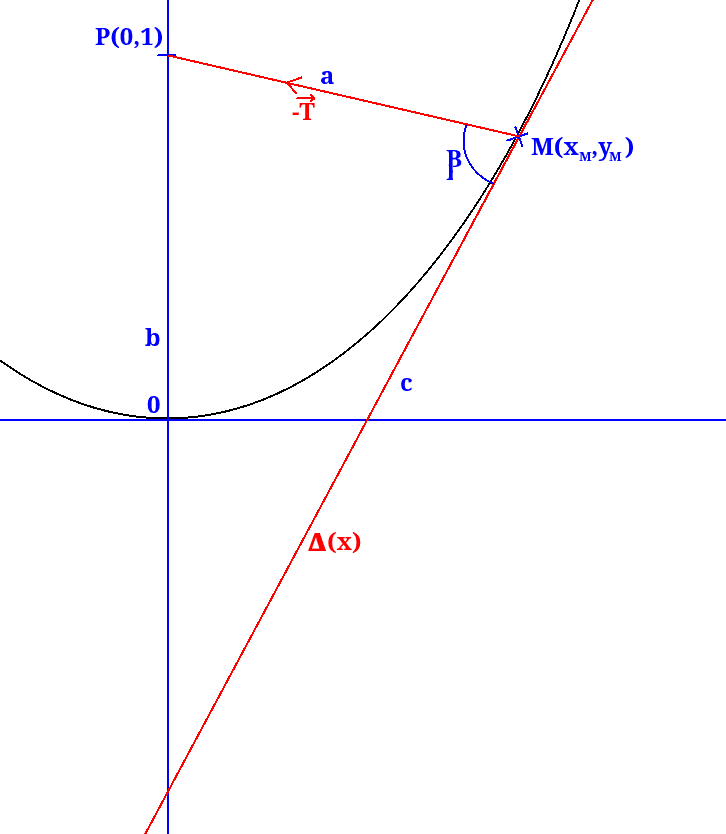
\includegraphics[scale=0.5]{al-kashi.png}
	%\caption{Histoire de Sanofi}
\end{figure}
On note x,y les coordonnées du point M.\\
$a=\sqrt{(x_M-x_P)^2+(y_M-y_P)^2}=\sqrt{x^2+(\frac{x^2}{2}-1)}=\sqrt{x^2+\frac{x^4}{4}-x^2+1}=\sqrt{\frac{x^4}{4}+1}$\\
$b=\sqrt{(x_M-x_P)^2+(y_M-\Delta(0))^2}=\sqrt{x^2+(\frac{x^2}{2}+\frac{x^2}{2})^2}=\sqrt{x^2+x^4}=x\sqrt{1+x^2}$\\
note : faut-il mettre plutôt $|x|\sqrt{1+x^2}$ ?\\
$c=\sqrt{(y_p-\Delta(0))^2}=\sqrt{(1+\frac{x^2}{2})^2}=1+\frac{x^2}{2}$\\
D'après le théorème d'Al-Kashi : 
$x_1 = \frac{5 + \sqrt{25 - 4 \times 6}}{2} = 3$\\
$c^2 = a^2 + b^2 - 2ab\times\cos(\beta)$\\
$\cos(\beta)=\frac{a^2+b^2-c^2}{2ab}=\frac{x^4/4+1+x^2+x^4-1-x^2-x^4/4}{2x\sqrt{x^4/4+1}\sqrt{1+x^2}}=\frac{x^3}{2\sqrt{\frac{x^4}{4}+1}\sqrt{1+x^2}}$\\
On trouve donc :
\[\fbox{ $T_t=T\times\frac{x^3}{2\sqrt{\frac{x^4}{4}+1}\sqrt{1+x^2}}$ }\]\\

\subsection{Determination de $ \|T\| $}
On détermine la valeur de la tension du ressort.\\
$T=k(l-l_0)=k(\sqrt{(x_M-x_P)^2+(y_M-y_P)^2}-l_0)=k(\sqrt{x^2+(x^2/2-1)^2}-l_0)$\\
$T=k(\sqrt{x^2+x^4/4-x^4+1}-l_0)$\\
\[\fbox{ $T=k(\sqrt{1+\frac{x^4}{4}}-l_0)$ }\]

\subsection{Détermination de $a_t$}
On a vu dans la première équation que $a_n=0$. On en déduit: $||\vec{a}||=a_t$\\
Avec une accélération normale nulle, on peut écrire la formule de l'accélération dans le repère de Frenet ainsi : $a_t=||\vec{a}||$\\ %=$\sqrt{a_x^2+a_y^2}$
Or $||\vec{a}||=\frac{\partial v}{\partial t}=\frac{\partial \pm\sqrt{\dot{x}^2+\dot{y}^2}}{\partial t}$\\
$ \dot{y}=\frac{\partial y}{\partial t}=\frac{\partial y}{\partial x}\times\frac{\partial x}{\partial t}=x\dot{x} $\\
$ v=\sqrt{\dot{x}^2+\dot{x}^2x^2}=\dot{x}\sqrt{1+x^2} $\\
$ \frac{\partial v}{\partial t}=\ddot{x}\sqrt{1+x^2}+\frac{\dot{x}^2x}{\sqrt{1+x^2}} $\\
On trouve: \[\fbox{$a_t=\ddot{x}.\sqrt{1+x^2}+ \frac{\dot{x}^2.x}{\sqrt{1+x^2}}$}\] (Equation de Charles)
%On obtient alors: $a_t=\sqrt{\ddot{x}^2+\ddot{y}^2}$

\subsection{Détermination de l'équation différentielle}
A l'aide de ce qu'on a calculé précédemment on développe l'équation $mg_t+T_t=ma_t$ pour déterminer l'équation différentielle.
On obtient alors: 
\subsubsection{Equa diff de Guillaume}
En développant et en prenant k=m, g=1 et $a=l_0$ (données de l'énoncé), on obtient :\\
$m.1.\frac{x}{\sqrt{1+x^2}} + m(\sqrt{x^4/4+1}-a).[\frac{1}{\sqrt{1+x^2}}.\frac{x}{\sqrt{1+x^4/4}} + \sqrt{1-\frac{1}{1+x^2}}.\sqrt{1-\frac{x^2}{1+x^4/4}}] - m.\ddot{x}.\sqrt{1+x^2} - m.\frac{\dot{x}^2.x}{\sqrt{1+x^2}} = 0$ \\
 
$\frac{x}{\sqrt{1+x^2}} + (\sqrt{x^4/4+1}-a).[\frac{1}{\sqrt{1+x^2}}.\frac{x}{\sqrt{1+x^4/4}} + \sqrt{1-\frac{1}{1+x^2}}.\sqrt{1-\frac{x^2}{1+x^4/4}}] - \ddot{x}.\sqrt{1+x^2} - \frac{\dot{x}^2.x}{\sqrt{1+x^2}} = 0$
  
$\frac{x}{\sqrt{1+x^2}} + (\sqrt{x^4/4+1}-a).[\frac{1}{\sqrt{1+x^2}}.\frac{x}{\sqrt{1+x^4/4}} + \frac{x}{\sqrt{1+x^2}}.\sqrt{\frac{x^4/4-x^2+1}{1+x^4/4}}] - \ddot{x}.\sqrt{1+x^2} - \frac{\dot{x}^2.x}{\sqrt{1+x^2}} = 0$
  
$\frac{x}{\sqrt{1+x^2}} + [\frac{x}{\sqrt{1+x^2}} + \frac{x.\sqrt{x^4/4-x^2+1}}{\sqrt{1+x^2}}] -a.[\frac{1}{\sqrt{1+x^2}}.\frac{x}{\sqrt{1+x^4/4}} + \frac{x}{\sqrt{1+x^2}}.\sqrt{\frac{x^4/4-x^2+1}{1+x^4/4}}] - \ddot{x}.\sqrt{1+x^2} - \frac{\dot{x}^2.x}{\sqrt{1+x^2}} = 0$
 
$\frac{x}{1+x^2} + [\frac{x}{1+x^2} + \frac{x.\sqrt{x^4/4-x^2+1}}{1+x^2}] -a.[\frac{x}{(1+x^2).\sqrt{1+x^4/4}} +\frac{x.\sqrt{x^4/4-x^2+1}}{(1+x^2).\sqrt{1+x^4/4}}] - \ddot{x} - \frac{\dot{x}^2.x}{1+x^2} = 0$

$\frac{2x+x.\sqrt{x^4/4-x^2+1}-\dot{x}^2.x}{1+x^2} -a.\frac{x+x.\sqrt{x^4/4-x^2+1}}{(1+x^2).\sqrt{1+x^4/4}} - \ddot{x}= 0$

$-\frac{2x+x.\sqrt{x^4/4-x^2+1}-\dot{x}^2.x}{1+x^2} +a.\frac{x+x.\sqrt{x^4/4-x^2+1}}{(1+x^2).\sqrt{1+x^4/4}} + \ddot{x}= 0$

$-\frac{2x+x.\sqrt{(x^2/2-1)^2}-\dot{x}^2.x}{1+x^2} +a.\frac{x+x.\sqrt{(x^2/2-1)^2}}{(1+x^2).\sqrt{1+x^4/4}} + \ddot{x}= 0$

\[ \fbox{$\frac{-x^3/2-x+\dot{x}^2x}{1+x^2} + \frac{a.x^3}{2(1+x^2).\sqrt{1+x^4/4}} + \ddot{x}= 0$} \]
  
  
% \[mg.\cos(\tan^{-1}(x_0)) + k(l-l_0).\cos(\tan^{-1}(x_0) - \tan^{-1}(\frac{y_0-1}{x_0}))=\sqrt{\ddot{x}^2+\ddot{y}^2}\]
 %En développant on a:\[mg.\cos(\tan^{-1}(x)) + k(\sqrt{(x^2/2-1)^2+x^2}-l_0).\cos(\tan^{-1}(x) - \tan^{-1}(\frac{x^2/2-1}{x})) - \sqrt{\ddot{x}^2+1}=0\]

\subsubsection{Equa diff de Charles}
On calcule maintenant l'équatio ndifférentielle du système en s'aidant des résultats précédents.\\
On part de l'équation $ P_t+T_t=ma_t $\\
avec $T_t=k(l-l_0)$ et $P_t=-mg$\\
En développant les expression on obtient :\\
$k(\sqrt{x^4/4+1}-l_0)\times \frac{x^3}{2\sqrt{x^4/4+1}\sqrt{1+x^2}}-mg\frac{x}{\sqrt{1+x^2}}=m(\ddot{x}\sqrt{1+x^2}+\frac{\ddot{x}^2x}{\sqrt{1+x^2}})$\\
$ \frac{k}{m}(\frac{x^3}{2\sqrt{1+x^2}}-\frac{x^3\times l_0}{2\sqrt{x^4/4+1}\sqrt{1+x^2}})-\frac{xg}{\sqrt{1+x^2}}-\ddot{x}\sqrt{1+x^2}-\frac{\dot{x}^2x}{\sqrt{1+x^2}}=0 $\\
En prenant k=m, g=1 et $a=l_0$ (données de l'énoncé), on obtient :\\
$ -\frac{x^3}{2\sqrt{1+x^2}}+\frac{x^3\times a}{2\sqrt{x^4/4+1}\sqrt{1+x^2}}+\frac{x}{\sqrt{1+x^2}}+\ddot{x}\sqrt{1+x^2}+\frac{\dot{x}^2x}{\sqrt{1+x^2}}=0 $\\
$ (-\frac{x^3}{2}+x)\frac{1}{2\sqrt{1+x^2}}+\frac{x^3\times a}{2\sqrt{x^4/4+1}\sqrt{1+x^2}}+\ddot{x}\sqrt{1+x^2}+\frac{\dot{x}^2x}{\sqrt{1+x^2}}=0 $\\
$ (-\frac{x^3}{2}+x)\frac{1}{2\sqrt{1+x^2}}+\frac{x^3\times a}{2\sqrt{x^4/4+1}\sqrt{1+x^2}}+\ddot{x}\sqrt{1+x^2}+\frac{\dot{x}^2x}{\sqrt{1+x^2}}=0 $\\
$ (-\frac{x^3}{2}+x)\frac{1}{1+x^2}+\frac{x^3\times a}{2\sqrt{x^4/4+1}(1+x^2)}+\ddot{x}+\frac{\dot{x}^2x}{\sqrt{1+x^2}}=0 $\\
\[ \fbox{$ \ddot{x}+\frac{\dot{x}^2x-x^3/2-x}{1+x^2}+\frac{x^3\times a}{2\sqrt{x^4/4+1}(1+x^2)}=0 $}\]

\section{Détermination des points d'équilibre}
Les points d'équilibre sont les points où la vitesse du système et donc de la masselotte est nulle. Ainsi, les tèrmes lié à la vitesse et à l'accélération du système sont nuls.\\
On part donc de l'équation :\\
$ \ddot{x}+\frac{\dot{x}^2x-x^3/2-x}{1+x^2}+\frac{x^3\times a}{2\sqrt{x^4/4+1}(1+x^2)}=0 $
où 
$\ddot{x}=\frac{\dot{x}^2x-x^3/2-x}{1+x^2}=0$\\
Ainsi on a :\\
$\frac{x^3\times a}{2\sqrt{x^4/4+1}(1+x^2)}=0$\\
En multipliant de part et d'autre de l'équation par $\frac{2(1+x^2)}{x}$ :\\
$x^2-\frac{x^2\times l_0}{\sqrt{1+x^4/4}}+2=0$
$\sqrt{1+x^\frac{4}{4}}(x^2+2)=x^2\times l_0$\\
$\sqrt{1+y^2}(2y+2)=2yl_0$\\
$(1+y^2)(4y^2+8y+4)=4y^2\times l_0^2$\\
$(1+y^2)(y^2+2y+1)=y^2\times l_0^2$\\
$(\frac{1}{y}+y)(y+2+\frac{1}{y})=l_0^2$\\
On pose $X=y+\frac{1}{y}$ ($y\neq 0$):\\
$X(X+2)=l_0^2$\\
$x^2+2X-l_0^2=0$\\
Dont on calcule le déterminant :
$\Delta_X=4(1+l_0^2)$\\
D'où les solutions intermédiaires :
$X_1=-1-\sqrt{1+l_0^2}$\\
$X_2=-1+\sqrt{1+l_0^2}$\\
$y+\frac{1}{y}=X$\\
$y^2+1=Xy$\\
$y^2-Xy+1=0$\\
Dont le déterminant est :
$\Delta_y=X^2-4$\\
D'où les solutions :
$y_1=\frac{1}{2}(X-\sqrt{X^2-4})$\\
$y_1=\frac{1}{2}(X+\sqrt{X^2-4})$\\
On peut alors trouver l'expression des points d'équilibre $y_1,y_2,y_3,y_4$ en fonction de $l_0$ :\\
$y_1=\frac{1}{2}(X_1-\sqrt{X_1-4})=\frac{-1-\sqrt{1+l_0^2}}{2}-\frac{1}{2}(\sqrt{(-1-\sqrt{1+l_0^2})-4})$\\
$=\frac{1}{2}(-1-\sqrt{1+l_0^2})-\frac{1}{2}\sqrt{1+2\sqrt{1+l_0^2}+(1+l_0^2)-4}$\\
$=\frac{1}{2}(-1-\sqrt{1+l_0^2})-\frac{1}{2}\sqrt{2+2\sqrt{1+l_0^2}+l_0^2-4}$\\
$y_2=\frac{X_1+\sqrt{X_1-4}}{2}=\frac{1}{2}(-1-\sqrt{1+l_0^2})+\frac{1}{2}\sqrt{2+2\sqrt{1+l_0^2}+l_0^2-4}$\\
$y_3=\frac{X_2-\sqrt{X_2-4}}{2}=\frac{-1+\sqrt{1+l_0^2}}{2}-\frac{1}{2}(\sqrt{(-1+\sqrt{1+l_0^2})-4})$\\
$=\frac{1}{2}(-1+\sqrt{1+l_0^2})-\frac{1}{2}\sqrt{1-2\sqrt{1+l_0^2}+(1+l_0^2)-4}$\\
$=\frac{1}{2}(-1+\sqrt{1+l_0^2})-\frac{1}{2}\sqrt{2-2\sqrt{1+l_0^2}+l_0^2-4}$\\
$y_4=\frac{1}{2}(-1+\sqrt{1+l_0^2})+\frac{1}{2}\sqrt{2-2\sqrt{1+l_0^2}+l_0^2-4}$\\
Il reste à déterminer la nature de ces points d'équilibre du système.

\section{Dans toute la suite on supposera que g=1, k=m et on notera $a=l_0$ et on s'intéressera particulièrement par l'équation vérifié par x(t).}
\subsection{Montrer que l'équation est de la forme: (E) $\ddot{x} + f(x,\dot{x},a) = 0$.}
\subsection{Déterminer en fonction de a les points d'équilibres du système.}
\subsection{Quelle est en fonction de a, la nature des points d'équilibres.}

\section{On suppose que $a=\sqrt{15}$.}
\subsection{Déterminer la valeur exacte des points d'équilibres du système.}
\subsection{Déterminer l'intégrale première du système.}
\subsection{Représenter le portrait de phase.}
\subsection{Que peut-on en déduire sur le mouvement.}

\section{On suppose maintenant que $a=\sqrt{3}$ et $x(0)=x_0>0$ et $\dot{x}(0)=0$.}
\subsection{Calculer et représenter à l'aide de Matlab la période T en fonction de $x_0$ pour $0<x_0<10$.}

\section{On suppose maintenant que le système est soumis à une force de frottement $\gamma > 0$ et que l'équation devient: (E) $\ddot{x} + \gamma.\dot{x} + f(x,a) = 0$.}
\subsection{Représenter le diagramme de Matlab le diagramme de bifurcation  en $(a,\gamma)$ pour chacun des points d'équilibres.}
\subsection{On suppose que $a=\sqrt{15}$. Pour quelles valeurs (exactes) de $\gamma$ les points d'équilibres attractifs changent-ils de nature.}
\subsection{Représenter le portrait de phase pour $\gamma=1, \gamma=2, \gamma=3.$}

\end{document} 